\section{Background and State of the Art}
\label{chapter:background}

\subsection{Representation of rotations}
\label{cha2:represent}
A 3D rotation can be represented in several ways, the most common are Euler angles and rotation matrices. Euler angles are three angles that define three rotations applied successively to three axes. Considering two 3D orthogonal right-handed coordinate systems, their relative orientation can be described by a $3\times3$ rotation matrix, $R$, which is parameterized by the Euler angles. There are many axes sequence conventions for Euler angles, in this work the convention will be ZYX, which corresponds to rotating around the torsional, vertical and horizontal axes. Considering a sequence of counter-clockwise rotations around Z axis by $\theta_Z$, resulting in the coordinate system Z'Y'X', around Y axis by $\theta_Y$, resulting in Z''Y''X'' and around X axis by $\theta_X$, resulting in Z'''Y'''X'''. 
The initial coordinate system is ZYX and the final coordinate system is Z'''Y'''X''', thus the rotation matrix can be defined as a multiplication (i.e. a serial order) of the following three rotation matrices, $R_Z$, $R_Y$ and $R_X$, noting that the order by which they are multiplied matters (rotations are non-commutative).
\begin{align}
\label{rrr}
R _ { z } ( \theta_Z ) = \left[ \begin{array} { c c c } { \cos \theta_Z } & { - \sin \theta_Z } & { 0 } \\ { \sin \theta_Z } & { \cos \theta_Z } & { 0 } \\ { 0 } & { 0 } & { 1 } \end{array} \right],\\ 
R _ { y } ( \theta_Y ) = \left[ \begin{array} { c c c } { \cos \theta_Y } & { 0 } & { \sin \theta_Y } \\ { 0 } & { 1 } & { 0 } \\ { - \sin \theta_Y } & { 0 } & { \cos \theta_Y } \end{array} \right], \\
R _ { x } ( \theta_X ) = \left[ \begin{array} { c c c } { 1 } & { 0 } & { 0 } \\ { 0 } & { \cos \theta_X } & { - \sin \theta_X } \\ { 0 } & { \sin \theta_X } & { \cos \theta_X} \end{array} \right],
\end{align}

\subsection{Camera Model}
\label{cha2:cameramodel}
It's possible to establish a relationship between a real point in space, $M_W = [X_W \ Y_W \ Z_W]^T$, and a point in an image in pixels, $\mathbf{m} = [u \ v]^T$, through the camera model as
\begin{equation}
 \lambda \mathbf{\widetilde{m}} \sim K [ R \ | \ \mathbf{t} ] \widetilde { M_W },
\end{equation}
where $\widetilde{\mathbf{m}}^T= [\mathbf{m}^T 1]$ and $\widetilde{\mathbf{M_W}}^T= [\mathbf{M_W}^T 1]$ are the, so called, homogeneous representations of $\mathbf{m}$ and $\mathbf{M_W}$, respectively.
The rotation $R$ and the translation $\mathbf{t}$ bring the point $M_W$, represented in the world reference frame to the camera's reference frame. $\lambda$ is a scale factor proportional to the depth of point $M$ in space. $K$ are the intrinsic parameters (focal length, $f$, meter to pixel scalings, $s_x$ and $s_y$, skew, $s$ and frame translation, $c_x$ and $c_y$) defined as
\begin{equation}
\label{sec2:eq:kmatrix}
K = \left[ 
\begin{array} { c c c } 
f s_x & s     & c_x \\ 
0 	  & f s_y & c_y \\ 
0     & 0     & 1   
\end{array} 
\right],
\end{equation} that bring the point from the image plane to the digital image. 
(Figure \ref{cha2:sec2:fig:camera_concepts}).   
\begin{figure}[ht]
	\centering
	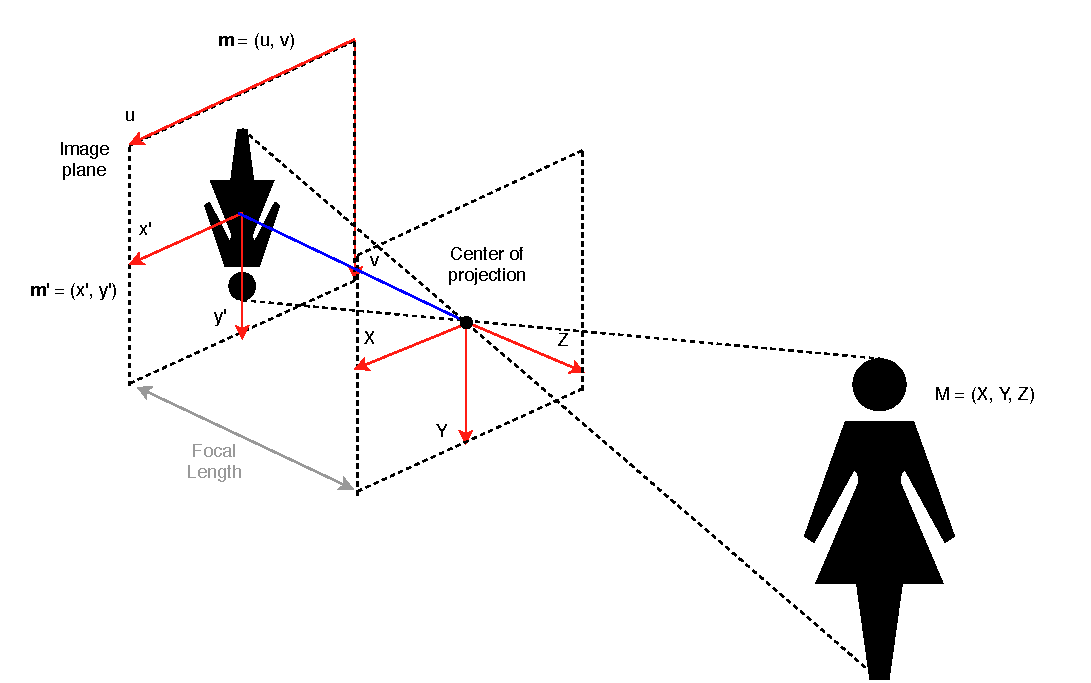
\includegraphics[width=0.5\textwidth]{images/cameraconcepts.pdf}
	\caption[Pinhole Camera Model]{Pinhole Camera Model. The girl defined by $M$ is projected onto the image plane defined by $\bf m$ through the light rays passing by the camera's pinhole. The focal length, $f$, is the length of the blue line. The digital image's coordinate system $(u, v)$ is defined on top right corner of the image plane, whereas the image plane is defined on the center.}
	\label{cha2:sec2:fig:camera_concepts}
\end{figure}


\subsection{Orthogonal Procrustes Problem}
\label{cha2:opprandsphere}
To estimate the difference in orientation, $R$, of a camera between two time instances $t_1$ and $t_2$ , there are several algorithms available in the literature. If the camera undergoes a pure rotation, a possible algorithm is using the solution to the Orthogonal Procrustes Problem (OPPR). This algorithm finds the optimal linear transformation between two 3D clouds of points, by minimizing the cost
\begin{equation}
\label{sec2:eq:procrustes}
\left \| M_2 - RM_1  \right \|^2 ,
\end{equation}
where $M_1$ into $M_2$ are the 3D coordinates of points in the environment measured in the reference frame of the camera at time $t_1$ and $t_2$, respectively. This problem can be solved by applying Singular Value Decomposition (SVD) to $M_1 M_2^T$, obtaining $R=V U^T$. \cite{procrustes} \\

However, in order to reconstruct the 3D point clouds from the images, it is necessary to have the depth of the point, $\lambda$, as seen on section \ref{cha2:cameramodel}, but this information is unavailable when using a single camera with unknown motion. Assuming pure rotation, any depth provides the same information, so it's possible to define an artificial depth by projecting the 2D points in a sphere with sufficient radius compared to the focal length, as follows
\begin{equation}
	\label{cha2:sec3:eq:spherepro}
	\left \| (\lambda \mathbf{m_1'})  \right \| = \left \| (\lambda x_1', \lambda y_1', \lambda)  \right \| = r
\end{equation}
where $m_1' = [ x_1' \ y_1']$ is a point on the image plane before rotating the camera, $r$ is the radius of the sphere and $\lambda$ then becomes
\begin{equation}
	\label{cha2:sec3:eq:lamdba}
	\lambda = \frac{r}{\sqrt{x_1'^2 + y_1'^2 + 1}}.
\end{equation}

Because OPPR only works for pure rotation, the translation associated (baseline constraint) is simply ignored.

\subsection{Epipolar Geometry}
\label{eppppp}
Epipolar geometry describes the relation between two images, before and after a transformation, through a 3x3 singular, non-invertible, matrix called the essential matrix, \textbf{$E$}, if the intrinsic parameters, $K$ are known, or the fundamental matrix, \textbf{$F$}, otherwise. It is expressed as 
\begin{equation}
\label{sec2:eq:epipolar}
\mathbf{\tilde{m}_2}^T F \mathbf{\tilde{m}_1} = 0,
\end{equation}
where ${m}_1$ and ${m}_2$ are pixel points in the image before and after rotating, respectively \cite{multiview}. 
From the fundamental matrix, $F$, it's possible to extract the rotation $R$ and the translation $\mathbf{t}$, through a somewhat complex factorization that yields
\begin{equation}
    F = K^{-T}[\mathbf{t}]_\times R K^{-1},
    \label{deewfwfe}
\end{equation}
where the essential matrix is $E = [\mathbf{t}]_\times R$. 
The fundamental matrix itself can be estimated through several methods. In Zhang's 1996 review on the issue \cite{detep}, the conclusion was that linear techniques are usually sensitive to noise and not very stable, because they ignore the constraints of $F$ and the minimization criterion is not physically meaningful. However, the results could be improved by using normalized data points instead of pixel coordinates. Three nonlinear algorithms are mentioned in the review paper: (i) determines the maximum likelihood estimation of the fundamental matrix, (ii) minimizes the symmetric epipolar error, and (iii) minimizes the first order geometric error. The first one is the most time-consuming. From the other two promising approaches, the second seems to give the worst results and the last algorithm has been proposed to give the best results in the least amount of computational time. \\

Algorithm (i) finds the maximum likelihood estimation of $F$ by minimizing the distances between the points in the image and its re-projections. Having $M_1$ as a point in space, the corresponding points in the images before and after rotating are $\widetilde{\mathbf{m}}_{1}$ and $\widetilde{\mathbf{m}}_{2}$, respectively, obtained through the camera model.
The re-projections of $\widetilde{\mathbf{m}}_{1}$ and $\widetilde{\mathbf{m}}_{2}$ are given by the projection functions $h_1(M_1, \mathbf{f})$ and $h_2(M_1, \mathbf{f})$, respectively, explained in Section 5.5 of Zhang 1996 \cite{detep}, where $\mathbf{f}$ is the vectorized fundamental matrix, $[f_{11} \ f_{12} \ f_{13} \ f_{21} \ f_{22} \ f_{23} \ f_{31} \ f_{32} \ f_{33}]^T$.

Algorithm (ii) minimizes the epipolar error symmetrically, which is the distance from a point to its epipolar line\footnote{See section 2.2 of Zhang 1996. \cite{detep}}.The epipolar line of the first image is defined as $\widetilde{\mathbf{l}}_{e_1} =  F\widetilde{\mathbf{m}}_{2}$ and the second's as $\widetilde{\mathbf{l}}_{e_2} =  F\widetilde{\mathbf{m}}_{1}$, the quantity to minimize is given by
\begin{equation}
	\min _{\mathbf{F}} \sum_{i}\left(d^{2}\left(\mathbf{m}_{2i}, \mathbf{l}_{e_{2}}\right)+d^{2}\left(\mathbf{m}_{1i}, \mathbf{l}_{e_{1}}\right)\right),
\end{equation}
where $d\left(\mathbf{p}, \mathbf{l}\right)=\frac{a p_{1}+b _{2}+c}{\sqrt{a^{2}+b^{2}}}$, with $\widetilde{\mathbf{l}} = (a, b, c)^{T}$
and $\mathbf{p}=\left(p_{1}, p_{2}\right)^{T}$, is the distance of a point to a line.\\

Minimizing the epipolar relation $ \sum_i (\mathbf{\widetilde{m_i}}'^T F \mathbf{\widetilde{m_i}})^2$ doesn't yield a good result because the variance of each $i$ term is not the same and the least-squares technique produces an optimal solution if each term has the same variance. So one possibility is to determine the fundamental matrix the way it's given by algorithm (iii) that minimizes:
\begin{equation}
\min_F \sum_i \frac{ (\mathbf{\widetilde{\mathbf{m}}_{2i}}^T F \widetilde{\mathbf{m}}_{1i})^2}{\sigma_i^2},
\end{equation}
where $\sigma_i^2$ is the variance given by 
\begin{equation}
\sigma_i^2 = \sigma [l_{{e1i}_x}^2 + l_{{e1i}_y}^2 + l_{{e2i}_x}^2 + l_{{e2i}_y}^2].
\end{equation}
This corresponds to minimizing the derivative of the epipolar relation, thus is also called Gradient-Based Technique (GRAT), or the Sampson error.
Because multiplying each term by a constant makes no difference, $\sigma$ can be dropped.\\

A disadvantage of epipolar geometry is that if the eye movement is not constrained by a translation component, the epipolar relation will not work, since $[\mathbf{t}]_\times$ would be a $3\times3$ matrix of zeros and, consequently, $E = [\mathbf{t}]_\times R$ would yield the same, making it impossible to retrieve the rotation.\\

\subsection{Robust Estimation}
\label{feinereg}
Wrongly matched pairs of points between the two images, or points with large location errors, can severely affect the precision of the rotation estimation. The reason for this is that all methods are least-square techniques that assume the noise which corrupts the data has zero mean. Hence, it is relevant to look into techniques of robust estimation.

In computer vision, it is very common to estimate the parameters of a model from image data. Robust estimation eliminates noise from the data. Points that don’t conform to a model are called outliers and are eliminated.

One technique of robust estimation, is RANdom SAmple Consensus (RANSAC), first introduced by Martin A. Fischler and Robert C. Bolles in 1981 \cite{ransac}, where a small set of inliers is used to find a model and test all the other points against it. In this manner, it's possible to discover which points fit the model or not, and if they don’t consider them outliers. The final model is the one that has the most inliers. 

However, it is necessary to first define the said model. In the present study, the model could be obtained with the OPPR applied to the point matches. More specifically, 3 point matches would suffice to estimate the rotation between images that, applied to the remaining matches, could define which ones are outliers or inliers, leading to more matching accuracy.

Besides the accuracy, there is another interesting effect produced using this technique:

\begin{enumerate}
\item Points that are closer to the camera are the ones that are more affected by the baseline constraint. The ones further way are a closer fit to pure rotations.

\item OPPR derives pure rotations as explained in section \ref{cha2:opprandsphere}. 
\end{enumerate}
Therefore by using RANSAC and OPPR together, points matches closer to the camera, are naturally eliminated. This corresponds to image sections that would be more affected by translation and might prove beneficial to eliminate them. \cite{mono} \\

